\documentclass[aspectratio=169]{beamer}
\usetheme{Madrid}
\usecolortheme{default}
\usepackage{graphicx}
\usepackage{booktabs}
\usepackage{hyperref}
\usepackage{tikz}
\usetikzlibrary{positioning, arrows.meta, petri, shapes.geometric, arrows, fit, backgrounds}

\graphicspath{{images/}}

\title[ByteRoute]{ByteRoute: Real-Time Network Traffic Monitoring}
\subtitle{Applicazioni e Servizi Web}
\author[Babini Stefano]{
    Babini Stefano \\
    \small 0001125127 \\
    \footnotesize \texttt{stefano.babini5@studio.unibo.it}
}
\institute[Unibo]{University of Bologna}
\date{\today}

\begin{document}

% Slide 1: Title
\begin{frame}
    \titlepage
\end{frame}

% Slide 2: Agenda
\begin{frame}{Agenda}
    \tableofcontents
\end{frame}

% ─────────────────────────────────────────────
\section{Introduction \& Problem Statement}
% ─────────────────────────────────────────────

\begin{frame}{What is ByteRoute?}
    \textbf{ByteRoute} is a real-time network traffic monitoring platform.
    \vspace{0.4cm}
    \begin{itemize}
        \item Captures network packets at the OS level on Linux via \texttt{libpcap}.
        \item Enriches records with geographic and organisational metadata (GeoIP, ASN).
        \item Presents results through an interactive web dashboard with live updates.
        \item Targets developers, system administrators, and security researchers.
    \end{itemize}
    \vspace{0.4cm}
    \textit{Built as a pnpm monorepo: Go client + Node.js backend + Vue.js~3 dashboard,
    all orchestrated with Docker Compose.}
\end{frame}

\begin{frame}{The Problem}
    Modern network activity is opaque and hard to reason about.
    \vspace{0.4cm}
    \begin{itemize}
        \item \textbf{Lack of visibility:} No easy way to see which countries or autonomous
              systems a host is contacting.
        \item \textbf{Fragmented tooling:} \texttt{tcpdump} and Wireshark require deep
              expertise; they produce no persistent, enriched records.
        \item \textbf{No multi-host correlation:} Monitoring several machines in a single
              unified view is impractical with existing CLI tools.
        \item \textbf{High barriers:} Enterprise solutions are expensive; self-hosted
              alternatives demand heavy infrastructure.
    \end{itemize}
\end{frame}

\begin{frame}{The Solution --- Three-Tier Architecture}
    \begin{enumerate}
        \item \textbf{Linux Client (Go):} Captures packets, aggregates them into connection
              records, and forwards batches over HTTPS with bearer authentication.
        \item \textbf{Backend (Node.js / Express):} Enriches data with GeoLite2, upserts
              into MongoDB, and broadcasts live updates via Socket.IO.
        \item \textbf{Dashboard (Vue.js~3):} Interactive SPA with a world map, live
              connection list, and real-time aggregated statistics.
    \end{enumerate}
    \vspace{0.4cm}
    \textit{Everything is containerised with Docker and exposed through a Traefik reverse
    proxy; the full stack starts with a single \texttt{docker compose up -d}.}
\end{frame}

% ─────────────────────────────────────────────
\section{Requirements}
% ─────────────────────────────────────────────

\begin{frame}{Functional Requirements}
    \begin{itemize}
        \item \textbf{Packet capture \& deduplication:} Derive 5-tuple connection records;
              deduplicate by full flow or by IP pair.
        \item \textbf{Batching:} Aggregate records respecting configurable limits on count
              and payload size before shipping to the backend.
        \item \textbf{Authenticated ingestion:} Accept batches only from clients presenting a
              valid bearer JWT.
        \item \textbf{GeoIP enrichment:} Resolve destination IPs to country, city,
              coordinates, ASN, and organisation via MaxMind GeoLite2.
        \item \textbf{Persistence:} Upsert enriched records into MongoDB, partitioned by
              tenant.
        \item \textbf{Real-time push:} Emit live connection updates and periodic statistics
              to the dashboard via Socket.IO.
        \item \textbf{Multi-tenancy:} Each user may own multiple tenants; data is always
              scoped and never crosses tenant boundaries.
        \item \textbf{Domain DSL:} Load a YAML config at startup to tune protocols,
              ingestion rules, and analytics queries without code changes.
    \end{itemize}
\end{frame}

\begin{frame}{Non-Functional Requirements}
    \begin{itemize}
        \item \textbf{Performance:} Backend handles continuous multi-agent ingestion without
              perceptible dashboard latency.
        \item \textbf{Security:} All \texttt{/api/*} endpoints protected by JWT; short-lived
              client tokens (default 12\,h) decouple agent credentials from user sessions.
        \item \textbf{Portability:} Server components run on any platform via Docker;
              the capture agent targets Linux due to \texttt{libpcap}.
        \item \textbf{Observability:} \texttt{GET /health} endpoint; CI publishes unified
              coverage reports for every pull request.
        \item \textbf{Maintainability:} pnpm workspaces + Turborepo enable independent
              versioning and testing of each package.
        \item \textbf{Scalability:} Tenant-partitioned data model accommodates multiple
              monitored hosts without schema changes.
    \end{itemize}
\end{frame}

% ─────────────────────────────────────────────
\section{Architecture \& Design}
% ─────────────────────────────────────────────

\begin{frame}{Deployment Topology}
\centering
\resizebox{0.88\textwidth}{!}{%
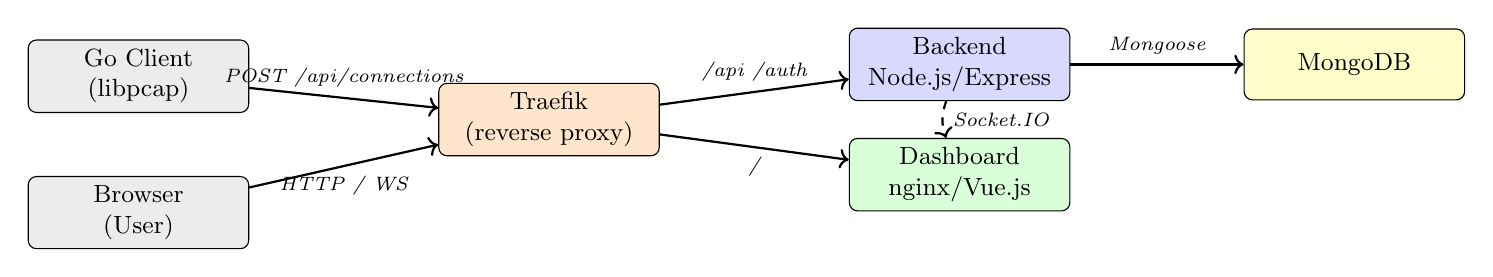
\begin{tikzpicture}[
    node distance=1.2cm and 1.4cm,
    box/.style={draw, rounded corners=3pt, minimum width=2.8cm, minimum height=0.9cm,
                font=\small, align=center},
    arr/.style={->, thick},
    lbl/.style={font=\scriptsize\itshape}
]
\node[box, fill=gray!15]  (client)   {Go Client\\(libpcap)};
\node[box, fill=gray!15, below=0.8cm of client] (browser)  {Browser\\(User)};
\node[box, fill=orange!20, right=2.4cm of client, yshift=-0.55cm] (traefik)  {Traefik\\(reverse proxy)};
\node[box, fill=blue!15,  right=2.4cm of traefik, yshift=0.7cm]  (backend)  {Backend\\Node.js/Express};
\node[box, fill=green!15, right=2.4cm of traefik, yshift=-0.7cm] (dashboard){Dashboard\\nginx/Vue.js};
\node[box, fill=yellow!20, right=2.2cm of backend] (mongo) {MongoDB};

\draw[arr] (client)  -- node[above, lbl]{POST /api/connections} (traefik);
\draw[arr] (browser) -- node[below, lbl]{HTTP / WS} (traefik);
\draw[arr] (traefik) -- node[above, lbl]{/api /auth} (backend);
\draw[arr] (traefik) -- node[below, lbl]{/} (dashboard);
\draw[arr] (backend) -- node[above, lbl]{Mongoose} (mongo);
\draw[arr, dashed] (backend) to[bend right=20] node[right, lbl]{Socket.IO} (dashboard);
\end{tikzpicture}%
}
\end{frame}

\begin{frame}{Backend Layered Architecture}
    Inspired by \textbf{Hexagonal Architecture (Ports \& Adapters)}:
    \vspace{0.3cm}
\centering
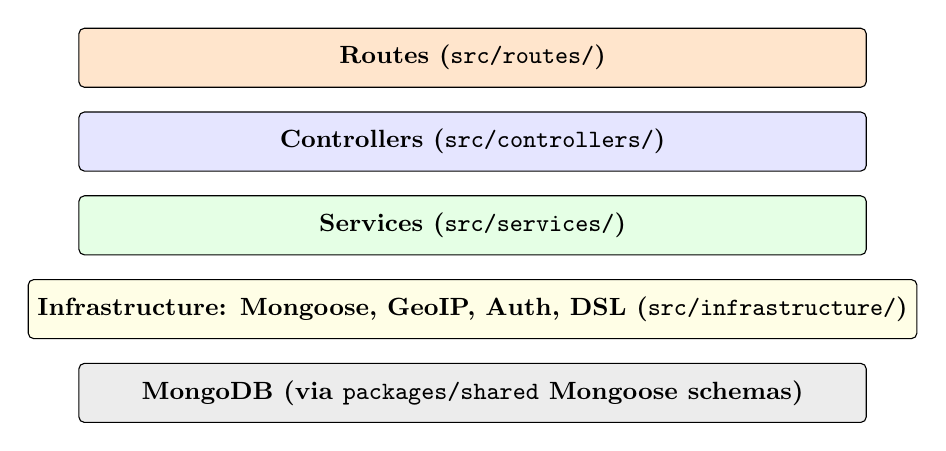
\begin{tikzpicture}[node distance=0.3cm]
\node[draw, rounded corners=2pt, minimum width=10cm, minimum height=0.75cm,
      font=\small\bfseries, align=center, fill=orange!20] (routes)
      {Routes (\texttt{src/routes/})};
\node[draw, rounded corners=2pt, minimum width=10cm, minimum height=0.75cm,
      font=\small\bfseries, align=center, fill=blue!10, below=of routes] (ctrl)
      {Controllers (\texttt{src/controllers/})};
\node[draw, rounded corners=2pt, minimum width=10cm, minimum height=0.75cm,
      font=\small\bfseries, align=center, fill=green!10, below=of ctrl] (svc)
      {Services (\texttt{src/services/})};
\node[draw, rounded corners=2pt, minimum width=10cm, minimum height=0.75cm,
      font=\small\bfseries, align=center, fill=yellow!10, below=of svc] (infra)
      {Infrastructure: Mongoose, GeoIP, Auth, DSL (\texttt{src/infrastructure/})};
\node[draw, rounded corners=2pt, minimum width=10cm, minimum height=0.75cm,
      font=\small\bfseries, align=center, fill=gray!15, below=of infra] (db)
      {MongoDB (via \texttt{packages/shared} Mongoose schemas)};
\end{tikzpicture}
\end{frame}

\begin{frame}{End-to-End Data Flow}
    \begin{enumerate}
        \item \textbf{Capture:} Go client opens a live \texttt{pcap} handle; BPF filter
              applied (user-supplied or auto-generated from local IPs).
        \item \textbf{Deduplicate:} Flow table keyed by 5-tuple (\texttt{flow}) or IP pair
              (\texttt{ip}); byte/packet counters incremented per record.
        \item \textbf{Batch \& flush:} On each tick idle flows are evicted; remaining records
              are split at \texttt{--max-batch-conns} / \texttt{--max-batch-bytes} bounds.
        \item \textbf{Ingest:} Batches posted to \texttt{POST /api/connections} with bearer
              JWT; tenant resolved from \texttt{X-Tenant-Id} header.
        \item \textbf{Enrich:} Domain DSL filters protocols; MaxMind resolves each
              destination IP to country, city, coordinates, ASN, and organisation.
        \item \textbf{Persist:} Bulk \texttt{updateOne} upserts into MongoDB
              (\texttt{tenantId + destIp} key).
        \item \textbf{Broadcast:} \texttt{connections:update} emitted via Socket.IO;
              statistics snapshot emitted every 30\,s.
        \item \textbf{Render:} Pinia stores updated reactively; map, list, and charts
              refresh without page reload.
    \end{enumerate}
\end{frame}

\begin{frame}{Domain Model}
    \begin{center}
    \begin{tabular}{lp{8.5cm}}
        \toprule
        \textbf{Entity} & \textbf{Description} \\
        \midrule
        \texttt{User}       & Authenticated platform user. Owns one or more tenants;
                               stores hashed credentials. \\
        \texttt{Tenant}     & Logical monitoring context (e.g.\ one per host). All
                               connection and metrics records are scoped to a tenant. \\
        \texttt{Connection} & Enriched connection record: source/destination IPs, port,
                               protocol, GeoIP data (country, city, coordinates, ASN,
                               organisation), timestamp, and status. \\
        \bottomrule
    \end{tabular}
    \end{center}
    \vspace{0.3cm}
    Schemas are centralised in \texttt{packages/shared} (Mongoose) to prevent
    model divergence between the backend and seeding scripts.
\end{frame}

\begin{frame}{Security \& Multi-Tenancy}
    \textbf{Authentication --- two token types (Passport.js + JWT)}
    \begin{itemize}
        \item \textbf{User JWT} (TTL: \texttt{1d}): issued at sign-up / sign-in;
              used by the dashboard and management API calls.
        \item \textbf{Client token} (TTL: \texttt{12h}): issued via
              \texttt{POST /auth/client-token}; used exclusively by the Go agent so the
              user's primary credential is never stored on a monitored host.
    \end{itemize}
    \vspace{0.4cm}
    \textbf{Tenant isolation}
    \begin{itemize}
        \item Every database query carries a \texttt{tenantId} filter.
        \item The backend rejects any attempt to read or write data for a tenant the
              authenticated user does not own.
        \item Socket.IO rooms are keyed by tenant ID; dashboards only receive events
              for their authorised tenant.
    \end{itemize}
\end{frame}

\begin{frame}{Domain DSL}
    A YAML file compiled once at startup governs two concern areas without code changes:
    \vspace{0.3cm}
    \begin{itemize}
        \item \textbf{\texttt{ingestion.connection}:} Allowed protocols
              (\texttt{TCP}, \texttt{UDP}, \texttt{ICMP}, \texttt{OTHER}), default protocol
              and status, optional source-IP deny list.
        \item \textbf{\texttt{analytics.queries}:} Sort field, order, and optional record
              limit for each statistics query (\texttt{byCountry}, \texttt{byAsn},
              \texttt{byProtocol}).
    \end{itemize}
    \vspace{0.3cm}
    \textbf{Resolution priority at container startup:}
    \begin{enumerate}
        \item \texttt{DOMAIN\_DSL\_PATH} environment variable.
        \item \texttt{/etc/byteroute/domain.dsl.yaml} (recommended Docker volume mount).
        \item \texttt{config/domain.dsl.yaml} relative to the working directory.
        \item \texttt{apps/backend/config/domain.dsl.yaml} --- bundled defaults.
    \end{enumerate}
\end{frame}

% ─────────────────────────────────────────────
\section{Technology Stack}
% ─────────────────────────────────────────────

\begin{frame}{Technology Stack}
    \begin{table}[]
        \centering
        \begin{tabular}{@{}ll@{}}
            \toprule
            \textbf{Component}   & \textbf{Technologies} \\ \midrule
            \textbf{Go Client}   & Go ($\ge$1.26), \texttt{gopacket/pcap} \\
            \textbf{Backend}     & TypeScript, Node.js, Express~5, Socket.IO, Mongoose \\
            \textbf{Dashboard}   & TypeScript, Vue.js~3, Vite, Pinia, Vue Router \\
            \textbf{Shared}      & TypeScript (Mongoose schemas, domain typings) \\
            \textbf{Auth}        & Passport.js (\texttt{passport-jwt}), HMAC-SHA256 JWTs \\
            \textbf{GeoIP}       & MaxMind GeoLite2 (City + ASN databases) \\
            \textbf{Infra}       & Docker, Docker Compose, Traefik~3.6, MongoDB~8 \\
            \textbf{CI/CD}       & GitHub Actions, semantic-release, pnpm, Turborepo \\ \bottomrule
        \end{tabular}
    \end{table}
\end{frame}

\begin{frame}{Web Stack Deep Dive}
    \textbf{Backend (Node.js / Express~5)}
    \begin{itemize}
        \item \texttt{express.json()} body parser capped at 2\,MB to match the client's
              \texttt{--max-batch-bytes} default.
        \item Socket.IO layered on the same \texttt{http.Server}: server-to-client push
              only (\texttt{connections:update} and aggregated statistics events).
        \item MongoDB bulk \texttt{updateOne} upserts keep ingestion latency low even under
              continuous multi-agent load.
    \end{itemize}
    \vspace{0.3cm}
    \textbf{Dashboard (Vue.js~3 SPA)}
    \begin{itemize}
        \item Composition API + \texttt{<script setup>} throughout; Pinia for state
              management (connections, statistics, auth, tenants).
        \item Vite dev server proxies \texttt{/api}, \texttt{/auth}, and
              \texttt{/socket.io} to the backend on port 4000 --- no CORS issues in
              development.
        \item Vue Router navigation guards redirect unauthenticated users to the login page.
    \end{itemize}
\end{frame}

% ─────────────────────────────────────────────
\section{Implementation Highlights}
% ─────────────────────────────────────────────

\begin{frame}{Go Client Internals}
    Internal packages under \texttt{apps/client-go/internal/}:
    \vspace{0.2cm}
    \begin{center}
    \small
    \begin{tabular}{lp{8cm}}
        \toprule
        \textbf{Package}  & \textbf{Responsibility} \\ \midrule
        \texttt{capture}  & Opens the pcap handle, applies BPF filter, decodes packets
                            into raw flow records. \\
        \texttt{flow}     & Maintains the in-memory flow table, deduplication, idle eviction. \\
        \texttt{backend}  & HTTP client: serialises batches to JSON and posts with bearer auth. \\
        \texttt{config}   & Parses CLI flags and env vars into a unified config struct. \\
        \texttt{metrics}  & Collects and periodically posts system and capture metrics. \\
        \texttt{util}     & IP parsing, BPF expression generation, shared helpers. \\ \bottomrule
    \end{tabular}
    \end{center}
\end{frame}

\begin{frame}{REST API Surface}
    \begin{center}
    \small
    \begin{tabular}{llp{5.5cm}}
        \toprule
        \textbf{Method \& Path}         & \textbf{Auth} & \textbf{Description} \\ \midrule
        \texttt{POST /auth/signup}       & No  & Create account; returns user JWT \\
        \texttt{POST /auth/signin}       & No  & Authenticate; returns user JWT \\
        \texttt{GET  /auth/me}           & Yes & Current user info \\
        \texttt{POST /auth/client-token} & Yes & Issue a short-lived agent token \\
        \texttt{GET  /api/tenants}       & Yes & List tenants owned by the user \\
        \texttt{POST /api/tenants}       & Yes & Create a new tenant \\
        \texttt{POST /api/connections}   & Yes & Ingest a batch of connections \\
        \texttt{GET  /api/connections/history} & Yes & Query stored connections \\
        \texttt{POST /api/metrics}       & Yes & Ingest metrics snapshots \\
        \texttt{GET  /health}            & No  & Returns \texttt{200 OK} when ready \\ \bottomrule
    \end{tabular}
    \end{center}
\end{frame}

\begin{frame}{Dashboard Features}
    \begin{itemize}
        \item \textbf{World map:} Visualises destination countries with pins and flow lines
              updating in real time as Socket.IO events arrive.
        \item \textbf{Live connection list:} IP, country, city, ASN, organisation, protocol,
              and status; refreshed without page reload.
        \item \textbf{Statistics panels:} Aggregated breakdowns by country, ASN, and
              protocol; time-series chart of connection volume.
        \item \textbf{Historical search (\texttt{/history-search}):} Full-text + structured
              query with status, protocol, and time-range filters; paginated via
              \texttt{limit} / \texttt{offset}.
        \item \textbf{First-run wizard:} Shown when the user has no tenants; guides through
              tenant creation and client-token generation; tested in both desktop and mobile
              viewports.
        \item \textbf{Tenant switcher:} Switch between monitored hosts without logging out.
    \end{itemize}
\end{frame}

% ─────────────────────────────────────────────
\section{Testing \& Quality}
% ─────────────────────────────────────────────

\begin{frame}{Testing Strategy}
    \textbf{Backend (Vitest)}
    \begin{itemize}
        \item \textbf{Unit tests:} Services, middleware, and domain logic in isolation;
              MongoDB and MaxMind replaced with mocks.
        \item \textbf{E2E tests:} Full Express app + MongoDB Memory Server; scenarios in
              Gherkin (\texttt{.feature} files) executed with Cucumber-JS covering auth,
              ingestion, tenants, and statistics.
    \end{itemize}
    \vspace{0.3cm}
    \textbf{Go Client}
    \begin{itemize}
        \item Unit tests accompany each internal package;
              \texttt{go test -coverprofile=coverage.out ./...} produces Cobertura XML.
    \end{itemize}
    \vspace{0.3cm}
    \textbf{Dashboard (Vitest + Playwright)}
    \begin{itemize}
        \item Browser-level checks run against Chromium, Firefox, WebKit, and a mobile
              Chromium viewport.
        \item Validates responsive layout, critical UI elements, and the first-run wizard
              flow; screenshots saved on failure.
    \end{itemize}
\end{frame}

\begin{frame}{CI/CD Pipeline (GitHub Actions)}
    Triggered on every PR and push to \texttt{main}:
    \vspace{0.3cm}
    \begin{enumerate}
        \item \textbf{Setup:} \texttt{pnpm install}, TypeScript type checking across the
              monorepo.
        \item \textbf{Parallel testing:}
        \begin{itemize}
            \item Backend unit + E2E tests (Vitest + MongoDB Memory Server).
            \item Dashboard component + browser tests (Vitest + Playwright matrix).
            \item Go client tests with coverage profile.
        \end{itemize}
        \item \textbf{Coverage consolidation:} Cobertura artifacts merged; summary
              published as a GitHub job annotation.
        \item \textbf{Semantic release:} Conventional commits drive version bump,
              \texttt{CHANGELOG.md} update, GitHub Release, and Docker image push to
              \texttt{ghcr.io}.
    \end{enumerate}
\end{frame}

% ─────────────────────────────────────────────
\section{Deployment}
% ─────────────────────────────────────────────

\begin{frame}{Docker Compose Stack}
    Four services defined in \texttt{docker-compose.yml}:
    \vspace{0.3cm}
    \begin{itemize}
        \item \textbf{Traefik~3.6:} Single public entry point on port 8080; routes by path
              prefix using Docker label rules (\texttt{/api}, \texttt{/auth},
              \texttt{/socket.io} $\to$ backend; \texttt{/} $\to$ dashboard).
        \item \textbf{MongoDB~8:} Health-checked; backend waits until ready before starting.
        \item \textbf{Backend:} Entrypoint downloads GeoLite2 databases automatically on
              first start; optional DSL volume mount at \texttt{/etc/byteroute/domain.dsl.yaml}.
        \item \textbf{Dashboard (nginx):} Pre-compiled Vue.js SPA; Nginx serves static
              assets.
    \end{itemize}
    \vspace{0.3cm}
    \textbf{Required environment variables:}
    \texttt{MAXMIND\_USER\_ID}, \texttt{MAXMIND\_API\_KEY}, \texttt{JWT\_SECRET}.
\end{frame}

% ─────────────────────────────────────────────
\section{Conclusion}
% ─────────────────────────────────────────────

\begin{frame}{Conclusion \& Future Work}
    \textbf{Achievements}
    \begin{itemize}
        \item Complete, end-to-end solution: Go capture agent $\to$ Node.js enrichment
              backend $\to$ Vue.js~3 real-time dashboard.
        \item Clean separation of concerns via multi-tenancy, Domain DSL, and layered
              backend architecture.
        \item Robust testing: unit, E2E (Gherkin/Cucumber), and cross-browser Playwright
              checks --- all gated in a single GitHub Actions workflow.
    \end{itemize}
    \vspace{0.3cm}
    \textbf{Future Directions}
    \begin{itemize}
        \item Cross-platform client (macOS, Windows) using platform capture APIs.
        \item Enhanced enrichment: RDAP or threat-intelligence feeds to label malicious IPs.
        \item Alert rules: threshold/pattern-based alerts with dashboard notifications.
        \item Horizontal scalability: Socket.IO Redis adapter to support multiple backend
              instances behind a load balancer.
    \end{itemize}
\end{frame}

\begin{frame}
    \centering
    \Huge \textbf{Thank You}
\end{frame}

\end{document}
